\begin{figure*}[ht!]
    \centering
    \begin{subfigure}[b]{0.3\textwidth}
         \centering
         % \includegraphics[trim={0 0 0 3cm},clip, width=\textwidth]{flash_bcop/figs/illustrations/block_conv_code_crop.png}
         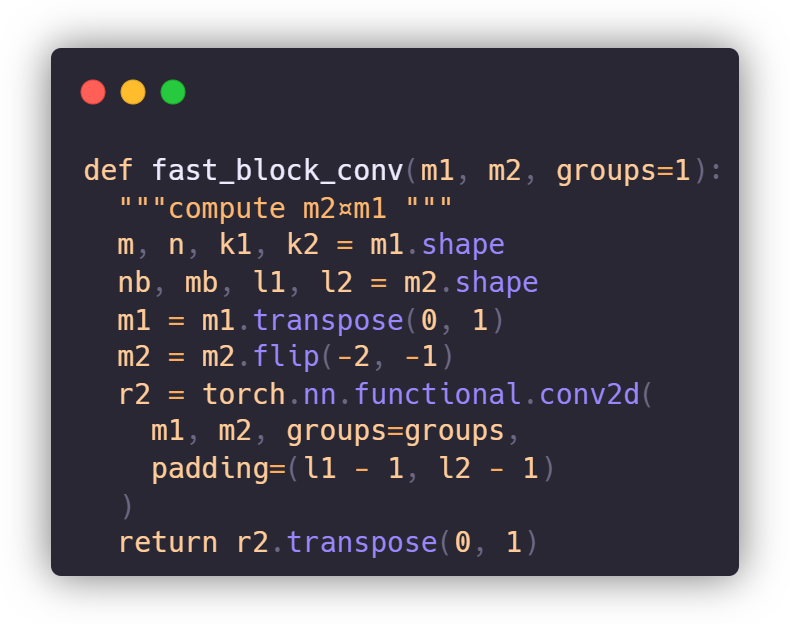
\includegraphics[width=\textwidth]{flash_bcop/figs/illustrations/block_conv_code_2.png}
         \caption{\textbf{Fast block convolution.} We optimized the 2D convolution in order to compute the $\mathbconv$ operator with maximum parallelism.}
         \label{fig:bconv_code}
    \end{subfigure}
    \hfill
    \begin{subfigure}[b]{0.43\textwidth}
         \centering
         %\includegraphics[width=\textwidth]{flash_bcop/figs/illustrations/parallel_associative_scan.drawio.png}
         %\includegraphics[width=\textwidth]{flash_bcop/figs/illustrations/parallel_bcop_v2.png}
         %\includegraphics[width=\textwidth]{flash_bcop/figs/illustrations/parallel_associative_scan_2.png} % with or without M at the end
         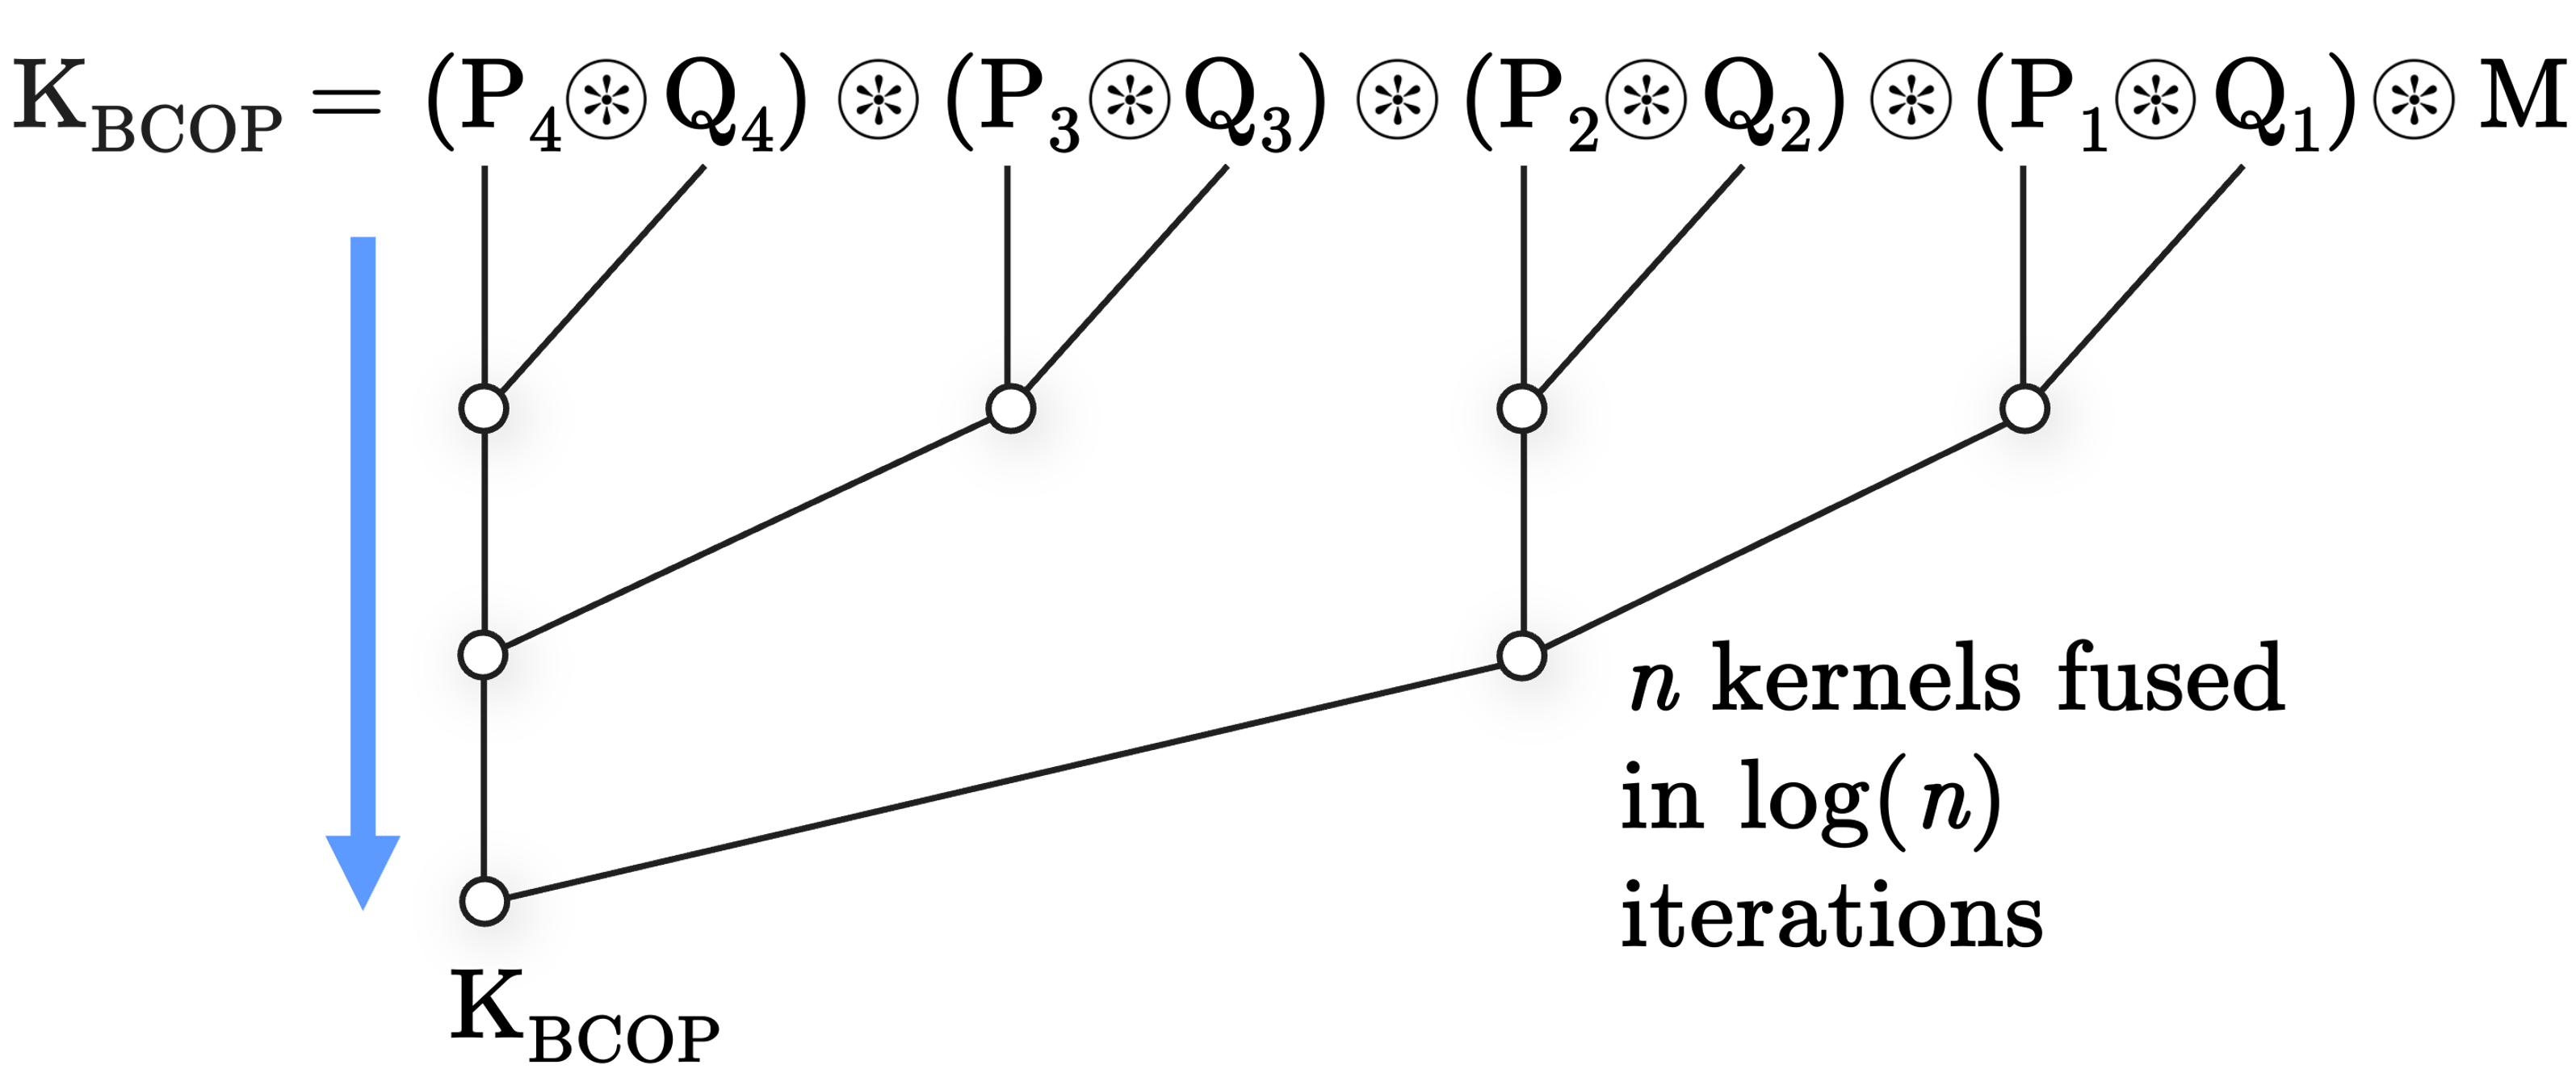
\includegraphics[width=\textwidth]{flash_bcop/figs/illustrations/parallel_v3.png}
         \vspace{3mm}
         \caption{\textbf{Parallelize BCOP iterations.} By leveraging associativity of $\mathbconv$, we can compute the $n$ iteration in $\mathcal{O}\log(n)$ steps using parallel associative scan.}
         \label{fig:bcop_pscan}
    \end{subfigure}
    \hfill
    \begin{subfigure}[b]{0.22\textwidth}
         \centering
         %\includegraphics[width=\textwidth]{flash_bcop/figs/illustrations/flowchart.drawio.png}
         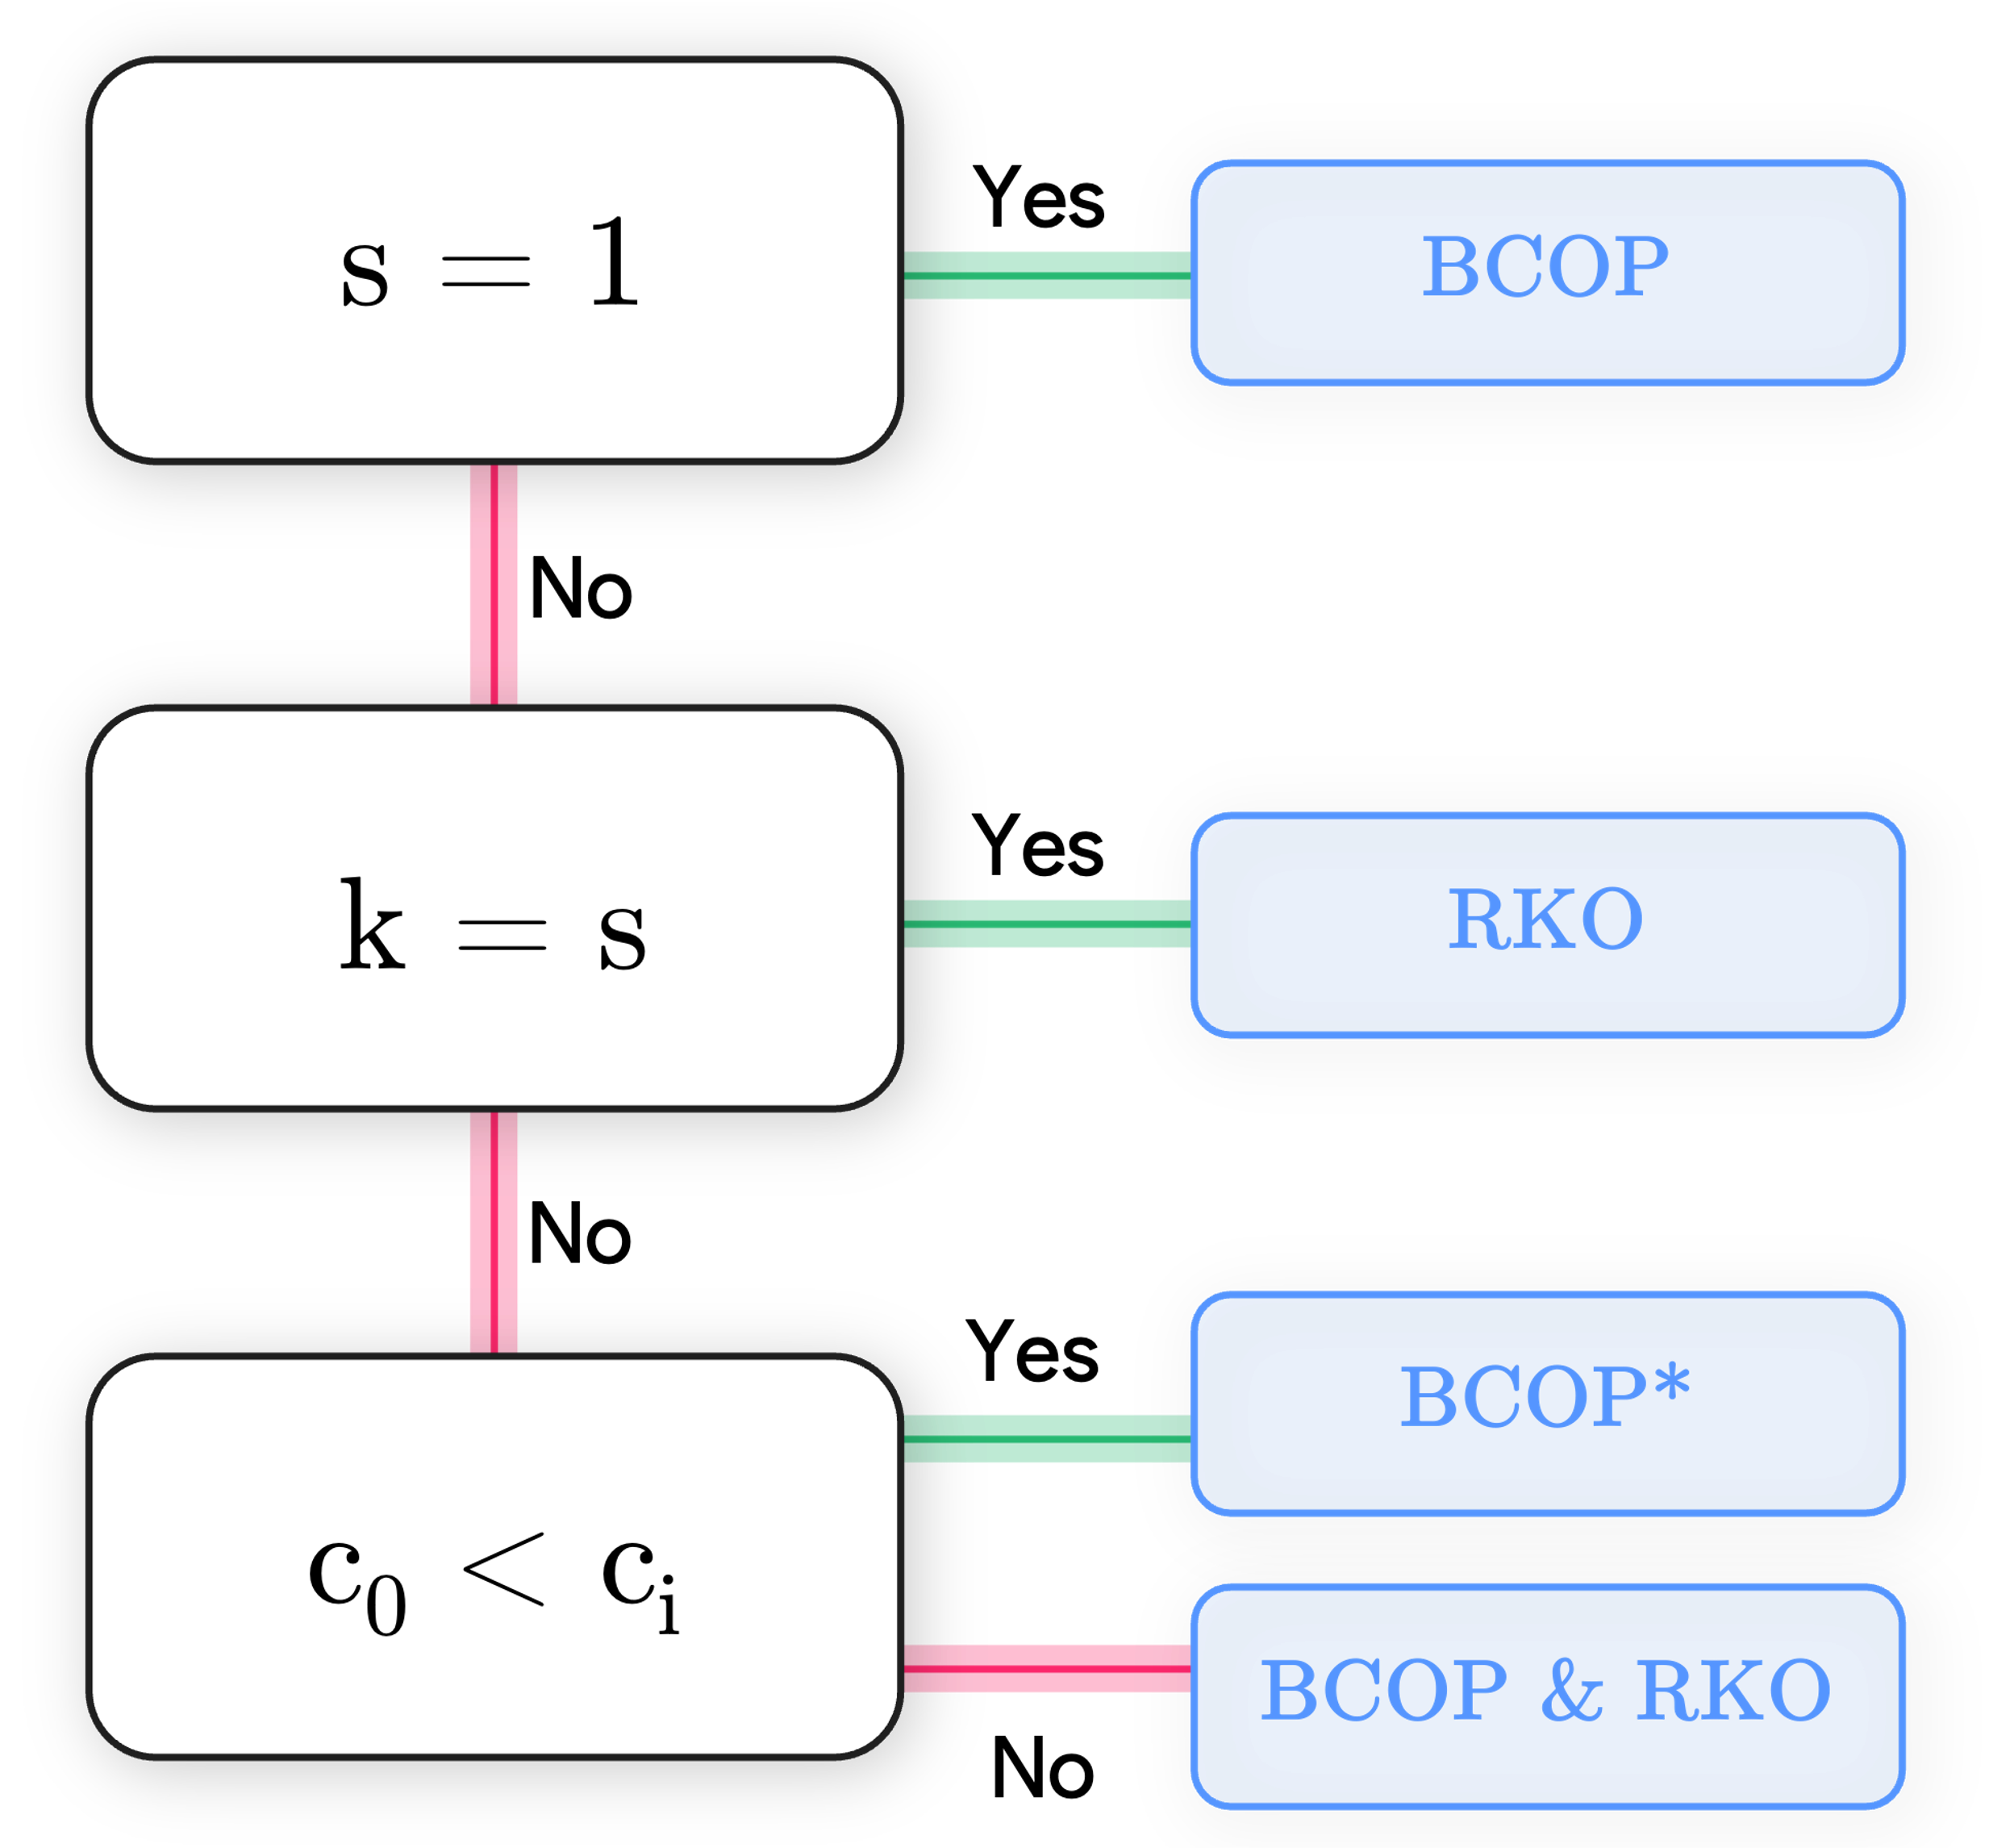
\includegraphics[width=\textwidth]{flash_bcop/figs/illustrations/flowchart_v4.png}
         % % \vspace{1mm}
         \caption{\textbf{Parsimonious parametrization.} The method can sometimes simplify to quicker equivalent parametrization.}
         \label{fig:method_simplify}
    \end{subfigure}
    \caption{\textbf{Fast implementation of AOC.} We achieve a highly scalable parametrization thanks to optimizations at every level of our method: starting from the $\mathbconv$ operator \ref{fig:bconv_code}, to BCOP \ref{fig:bcop_pscan}, to our complete method \ref{fig:method_simplify}. It results in a method with a lower overhead as scale increases.
    \vspace{-2mm}
    }
    \label{fig:optimizations}
\end{figure*}